% LaTeX file for resume 
% This file uses the resume document class (res.cls)

\documentclass[margin]{res} 
% the margin option causes section titles to appear to the left of body text 
\textwidth=5.2in % increase textwidth to get smaller right margin
\usepackage{helvetica} % uses helvetica postscript font (download helvetica.sty)
%\usepackage{newcent}   % uses new century schoolbook postscript font 
%\usepackage{url}
\usepackage{fontawesome}
\usepackage{graphicx}
\usepackage{hyperref}
\hypersetup{
    colorlinks=true,
    linkcolor=blue,
    filecolor=magenta,      
    urlcolor=cyan,
}
\urlstyle{same}


\begin{document} 
	
  % the \\[12pt] %adds a blank line after name
  \iffalse
  {\bf Avijit Bhattacharjee} 
 \begin{figure}
     %\centering
     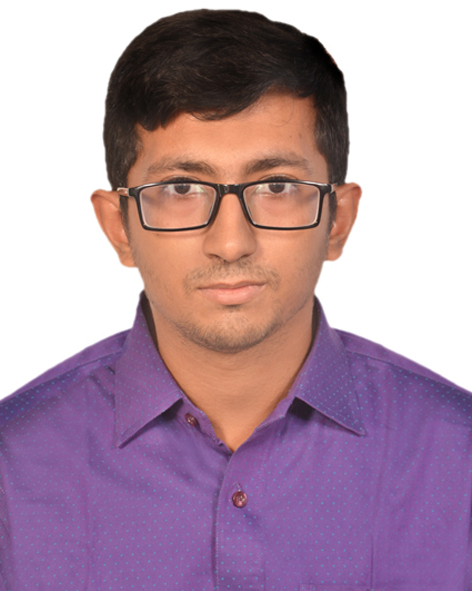
\includegraphics[width=2.75cm, height=3cm]{22}
     %\caption{Avijit Bhattacharjee}
     %\label{fig:my_label}
 \end{figure}
\fi 
\name{ Avijit Bhattacharjee\\[12pt]}
%\address{{\bf Present Address} \\ 50/b, South Jatrabari \\ %Dhaka-1204,Bangladesh \\
  %      Email : avijit.bhattacharjee@protonmail.com %\\
 %       Phone : +8801726512523}
%\address{{\bf Permanent Address} \\ 29 Runner Lane \\ Syosset, NY 11971 %\\
 %       (516) 921-7653 }


\begin{resume} 
 \begin{minipage}{0.30\linewidth}
    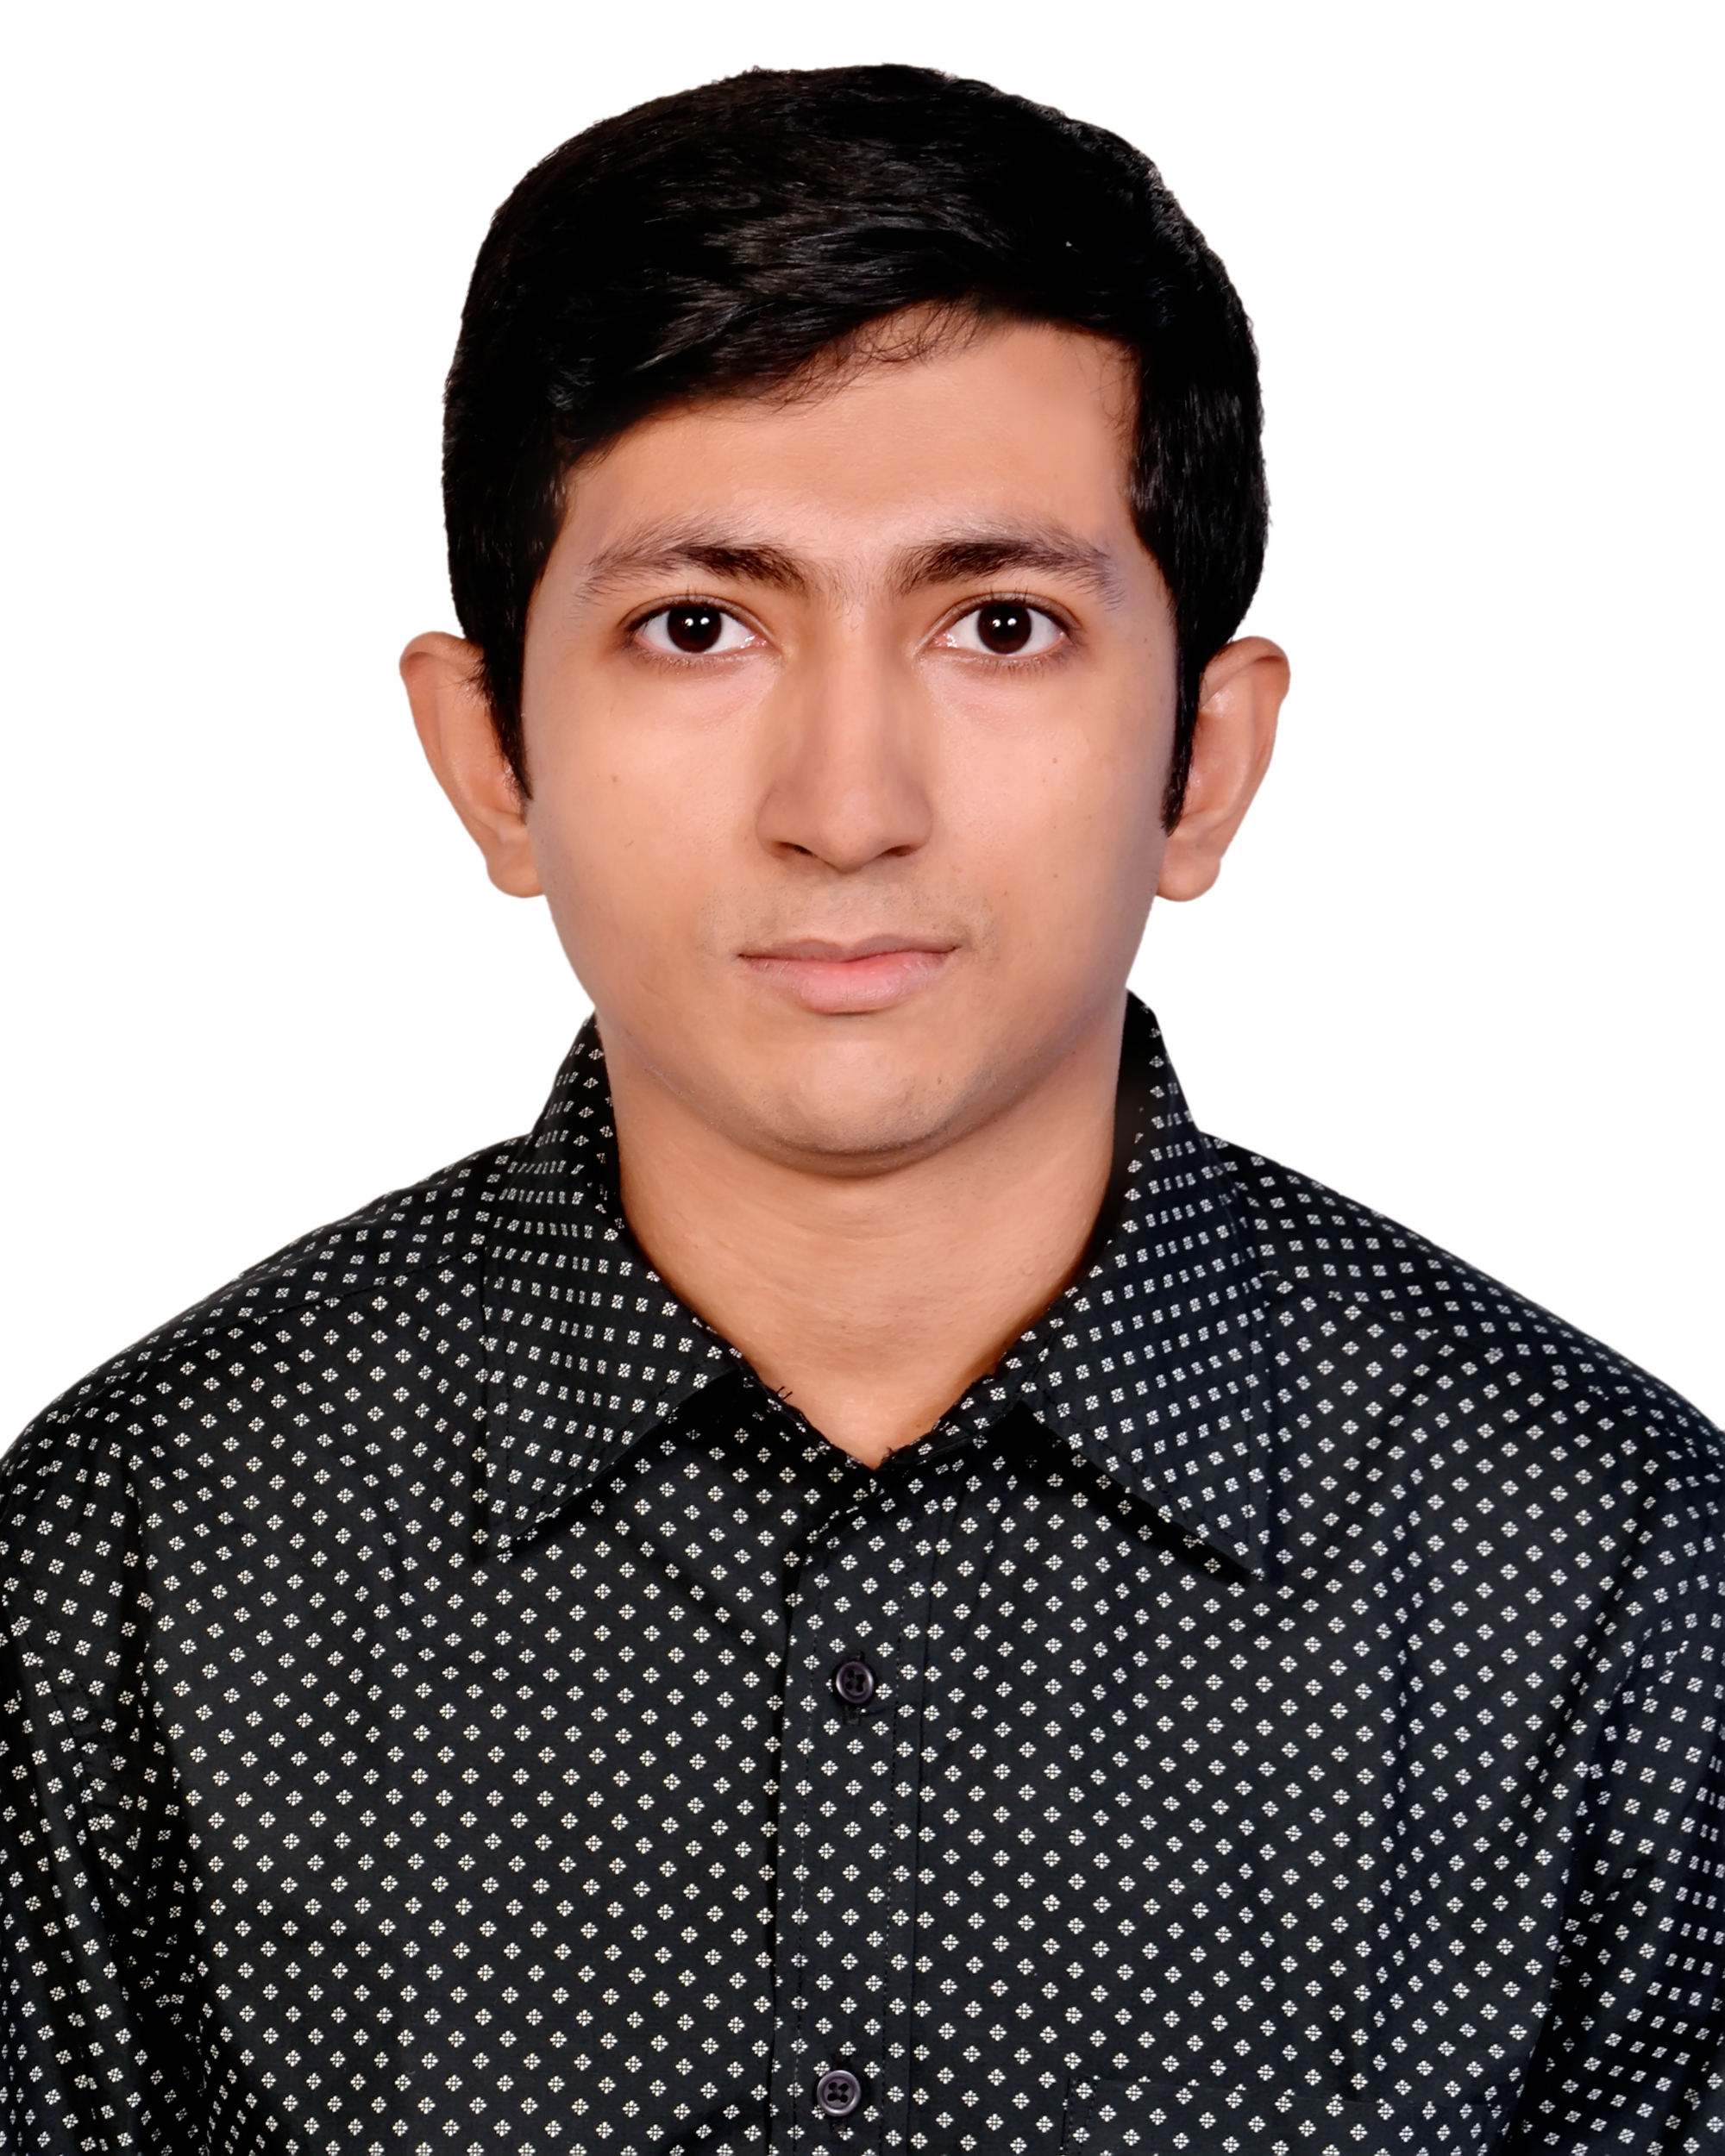
\includegraphics[width=2.75cm, height=3cm]{profile.jpg}\\
    \iffalse{}
 	\href{http://www.cseku.ac.bd/}{Khulna University}\\
 	Computer Science \& Engineering \\
 	Discipline\\
 	Satyendra Nath Bose Building \\
 	Gollamari, Khulna-9100\\
 	\fi
 \end{minipage}
 \begin{minipage}{0.45\linewidth}
 	\begin{tabular}{ll}
 		%Phone: & (+1) 3067139512 \\
 		Linkdein: &  \href{https://www.linkedin.com/in/avijit-bhattacharjee/}{avijitbhattacharjee} \\
 		Email: & \href{mailto:avijit.bhattacharjee@usask.ca}{\tt avijit.bhattacharjee@usask.ca}\\
 		Homepage: & \href{http://avijitbhattacharjee.com/}{\tt http://avijitbhattacharjee.com/} \\
 		Github: & \href{https://github.com/avijit1258}{\tt avijit1258}\\
 		%Address: & 206-103 Cumberland Ave S, S7N 1L5,\\ Saskatoon, Canada
 	\end{tabular}
 \end{minipage}
 
 \section{Summary}
 \begin{itemize} \itemsep -2pt
                 \item    Completed B.Sc. in CSE with CGPA 3.74 / 4.0 (2nd position in my batch)
                 \item    Participated in prestigious ICPC Dhaka Regional'2017 and NCPC'2015
                 \item    Former Vice-President of CLUSTER
                 \item    Completed few useful projects in Undergrad
                 \item    Organized CSE fest'2017, Study tour'2017 and volunteered to similar programs previously.
     \end{itemize}
 
\section{Education}
\textit{M.Sc. }, Computer Science(Software Research Lab) \hfill Jan 2019 - Present \\ University of Saskatchewan, Canada \\
Course average: 89\%\\

\textit{B.Sc. in Engg}, Computer Science And Engineering \hfill June 2014 - August 2018\\ Discipline, Khulna University, Khulna \\
CGPA 3.74 / 4.0 (2nd among 40 students) \\
\\
\textbf{ Thesis Title: ``Phylogenetic Tree Construction Using Chemical Reaction\\ Optimization''}

\textit{HSC} from Dhaka City College, Dhaka with GPA-5.0/5.0
 \hfill  2011 - 2013  
 
\textit{SSC} from Jatrabari Ideal High School, Dhaka with GPA-5.0/5.0
\hfill  2011
 \section{Research Interests} 
Software Engineering, Data Mining, Machine Learning, Cloud Computing, Optimization Problems

\section{Publications}
Bhattacharjee, Avijit, SK Rahad Mannan, and Md Rafiqul Islam. \textit{Phylogenetic Tree Construction Using Chemical Reaction Optimization.} International Conference on Intelligent Systems Design and Applications. Springer, Cham, 2018.\href{https://link.springer.com/chapter/10.1007/978-3-030-16660-1_89}{\faLink}

\section{Experience}

{\bf Graduate Teaching Assistant,} University of Saskatchewan 
\hfill Sept 2019 - Present
 \begin{itemize} \itemsep -2pt  % reduce space between items
 \item As a graduate teaching assistant, my role is to grade assignments, midterm and final exam papers. 
 
 \end{itemize}
 
 {\bf Graduate Research Assistant,} University of Saskatchewan 
 \hfill Jan 2019 - Aug 2019
 \begin{itemize} \itemsep -2pt  % reduce space between items
 \item Currently, I am working on modernizing a legacy system called \textit{CRHM: The Cold Regions Hydrological Model.}  CRHM is also part of mega project "GWF: Global Water Future". GWF is the most cited freshwater research program in the world which looks for solutions to Water Threats in an Era of Global Change.
 
 \end{itemize}

 {\bf Intern,} Trustaira Bangladesh Limited \hfill July 2017 - Aug 2017
 \begin{itemize} \itemsep -2pt  % reduce space between items
 \item Integrated several modules in order to analyze phonetic Bengali sentences.\href{https://techfoxweb.wordpress.com/2017/07/24/banglish-sentiment-analysis/}{\faWordpress }
 
 \end{itemize}
 
{\bf Vice-President,} CLUSTER \hfill  Jan 2017 - Dec 2017
\begin{itemize} \itemsep -2pt %reduce space between items
\item Club for Updated Search on Computer (CLUSTER) was established on 1999 by CSE Discipline, Khulna University. The club is well known all around the country for its IT-based social activities at the southern part of Bangladesh. 

\end{itemize}

 \section{Academic \\ Honors}
 
 \begin{itemize}
     \item University Merit List \hfill 2014- 2017 
     \item Faculty Stipend / Department Scholarship \hfill Sept 2019 - Present
     \item Faculty Stipend  \hfill Jan 2019 - Aug 2019
 \end{itemize}{}
 

\section{Competition Faced}
\begin{itemize} \itemsep -2pt
                 \item  ACM ICPC Dhaka Site Regional   \hfill Nov 2017 \\  
                orgranized by University Of Asia Pacific, Bangladesh
                 \item  BUET NCPC organized by Bandladesh \hfill 2015\\
                 University of Engineering and Technology
                 \item  ACM ICPC Dhaka Site Regional Preliminary  \hfill 2014-2017 \\  
                
     \end{itemize}

\iffalse
\section{Projects} 
               {\bf TouchTypeMaster,} Touch typing learning tool for windows   
                \begin{itemize} \itemsep -2pt
              \item \underline{Tools}:  Visual Studio, Microsoft Access Database,C\#                 
                \item  \underline{Description}:  Touch typing is a process which encourages to type using 10 fingers. This tool guides to learn typing at speed 60-90wpm. 

                \item \underline{Link}: \url{https://github.com/avijit1258/Touch-Type-Master}

		 \end{itemize}

		{\bf PIGEON,} Online Bus Ticket Booking System  
                \begin{itemize} \itemsep -2pt
                 \item  \underline{Tools}:  Laravel, Sublime Text, PHP 
                 \item  \underline{Description}:  PIGEON is a online bus ticketing  
                 system. 
                  \item \underline{Link}: \url{https://github.com/avijit1258/pigeon}                
                  
		 \end{itemize}

                  {\bf PMS, }  Project Management Software Like Trello 
                 \begin{itemize} \itemsep -2pt

               \item \underline{Tools}: Laravel, Sublime Text , PHP  
                 
                \item  \underline{Description}:  
                Motivation behind this project is ``Silicon Valley'' tv series. In an episode Jared shows Trello type concept on white board to organize tasks to two other members.  
              \item \underline{Link}: \url{https://github.com/avijit1258/PMS}
            
		 \end{itemize}

     {\bf Integer Computer Management Solutions,}   
                 \begin{itemize} \itemsep -2pt

               \item \underline{Tools}:  Laravel, Sublime Text, PHP, MySQL   
                 
                \item  \underline{Description}:  This project is a management solution for 
                Integer Computer Solutions, Khulna. They have a desktop application. We have built a web version for them in Software Engineering solution course.

               \item \underline{Link}: \url{https://github.com/avijit1258/Integer_Computershop_Management_Solution}
				
     \end{itemize}

     {\bf Online Admission Test Registration System,}   
                 \begin{itemize} \itemsep -2pt

               \item \underline{Tools}:  Sublime Text, PHP, MySQL, JQuery, Bootstrap   
                 
                \item  \underline{Description}:  For undergraduate admission test registration, every university in Bangladesh, needs an online registration system. As Web Programming Language project we have developed one for Khulna University admission test registration.


     \end{itemize}

     {\bf Numerical Methods Library}   
                 \begin{itemize} \itemsep -2pt

                \item \underline{Tools}:  codeblocks, c++, sublime text   
                 
                \item  \underline{Description}:  A library which includes implementation of important numerical methods such as false method, bisection method, secant method, gauss-siedel method, newton's divided difference etc.

                \item \underline{Link}:  \url{https://github.com/avijit1258/NumericalMethods}

     \end{itemize}

     {\bf Computer Graphics Library}   
                 \begin{itemize} \itemsep -2pt

                \item \underline{Tools}:  Codeblocks, C++, Sublime text,Ubuntu, vim, SDL-libgraph  
                 
                \item  \underline{Description}:  A library which includes implementation of important graphics algorithms such as Bressenhams algorithm, Cohen-shutherland algorithm etc.

                \item \underline{Link}:  \url{https://github.com/avijit1258/computer_graphics_lab}

                %\href{https://github.com/avijit1258/NumericalMethods}{NumericalMethods}

     \end{itemize}

      {\bf Online Judge Problem Solutions}   
                 \begin{itemize} \itemsep -2pt

                \item \underline{Sites}:  \href{https://uhunt.onlinejudge.org/id/586034}{UVA}(100+), \href{http://lightoj.com/volume_userstat.php?user_id=16115}{LightOJ}, \href{http://codeforces.com/profile/avijit1258}{Codeforces}   
                 
                \item  \underline{Description}: In my free time, I prefer to solve algorithm base teaser problems.

                \item \underline{Link}:  \url{https://github.com/avijit1258/CompetitiveProgramming}


     \end{itemize}

\fi


% Tabulate Computer Skills; p{3in} defines paragraph 3 inches wide
\section{Skills}
   \begin{tabular}{l p{3in}}
    \underline{Languages}: &  Python, C++, Java \\
     \underline{Software}: &  Git, VIM, Sublime text, Latex\\
	 \underline{Operating Systems}: & Linux, Windows\\
     \underline{Frameworks and Library}: & Bio++(A C++ library for bioinformatics), Laravel, Flask, GoJS, Scikit-learn
	
 \end{tabular}

\section{Undergraduate Projects}

\begin{tabular}{ l l}
    \textbf{Title} &  \textbf{Link} \\
     Touch-type learning application for windows & \href{https://github.com/avijit1258/Touch-Type-Master}{\faGithub} \\
    \\
     An Online Bus Ticket Booking System PIGEON & \href{https://github.com/avijit1258/pigeon}{\faGithub} \\
    \\
     Project Management Software Like Trello & \href{https://github.com/avijit1258/PMS}{\faGithub} \\
    \\
    Integer Computer Management Solutions & \href{https://github.com/avijit1258/Integer_Computershop_Management_Solution}{\faGithub} \\
    \\
    Online Admission Test Registration System for KU & \href{https://bitbucket.org/avijit1258/ku-ug-online-admission-test-registration-system/}{\faBitbucket} \\
    \\
     My Online Judge Problem Solutions &  \href{https://github.com/avijit1258/CompetitiveProgramming}{\faGithub } \\
    
\end{tabular}

 \section{Extra Curricular Activities}
\begin{itemize} \itemsep -2pt
    \item Member, Bridge City Bicycle Co-operative \href{https://bridgecitybicyclecoop.com}{\faGlobe }
    \item Coordinator, CSE Discipline Study Tour-2017
     \item  Organizing Member, KU CSE Fest 2017 
     \item Volunteer, KU CSE Fest 2015 
                
     \end{itemize}
     
     \section{References}
     \begin{itemize}
     	\itemsep -2pt
     	\item Dr. Chanchal Roy \\ Professor, University Of Saskatchewan \\Email: chanchal.roy@usask.ca
     	
     	\item Dr. Banani Roy \\ Assistant Professor, University Of Saskatchewan \\Email: banani.roy@usask.ca
     	
    %  	\item Dr. Md. Anisur Rahman\\ Professor, Khulna University \\Email: anis@cseku.ac.bd %\\ Phone: +8801927025032
    %  	\item Dr. Kamrul Hasan Talukder\\ Professor, Khulna University \\Email: k.h.t@alumni.nus.edu.sg %\\Phone: +8801925687763
     	%\item  Dr. Rameswar Debnath\\ Professor, Khulna University
     	%\\Email: rdebnath@cseku.ac.bd \\ Phone: +8801715182784 
     \end{itemize}

\end{resume} 
\end{document} 



